\documentclass[12pt,letterpaper]{article}

\usepackage[T1]{fontenc}
\usepackage[margin=1in,headheight=1.5em]{geometry}
\usepackage{enumitem}
\usepackage{fancyhdr}
\usepackage{lastpage}
\usepackage{float}
\usepackage{tabu}
\usepackage{booktabs}
\usepackage{graphicx}
\usepackage{lmodern}

\begin{document}

\renewcommand\headrule{}

\pagestyle{fancy}
\fancyhf{}
\lfoot{COMP 3004}
\rfoot{\thepage/\pageref{LastPage}}
\cfoot{Requirements Analysis Document}

% CUSTOM COMMANDS
\newcommand{\teamname}{Code First, Think Later}
\newcommand{\personone}{Kevin Hua}
\newcommand{\persontwo}{Hendrik Knoetze}
\newcommand{\personthree}{Juhandr\'e Knoetze}
\newcommand{\ccindent}{\hspace{1.5em}\hangindent=1.5em}
% END CUSTOM COMMANDS

% TABLE STYLING
\everyrow{\hline}
\tabulinesep=0.5em
\setlength\extrarowheight{0.5em}
% END TABLE STYLING

\thispagestyle{empty}

\begin{center}
	CARLETON UNIVERSITY
\end{center}

\vfill

\begin{center}
	{\fontsize{55pt}{55pt}\selectfont cuPID}
	\vspace{0.5em}\rule{\textwidth}{0.5pt}
	Requirements Analysis Document
\end{center}

\vspace{5em}

\begin{center}
	\textbf{Team [\teamname{}]}\\
	\personone{}\\
	\persontwo{}\\
	\personthree{}
\end{center}

\vfill

\begin{center}
	Submitted to:\\
	Dr. Christine Laurendeau\\
	COMP 3004: Object Oriented Software Engineering\\
	School of Computer Science\\
	Carleton University
\end{center}

\vspace{2em}

\begin{center}
	\today
\end{center}

\newpage{}

\tableofcontents{}

\renewcommand{\listfigurename}{Figures}
\listoffigures

\renewcommand{\listtablename}{Tables}
\listoftables

\newpage{}

\section{Introduction}

\begin{center}
    -- project --
\end{center}

\begin{center}
	\Huge [cuPID]
\end{center}

\begin{center}
    \rule{0.85\textwidth}{0.5pt}
\end{center}

\subsection{Purpose of System}

Team projects are typically assigned in University courses in order to develop and foster
good teamwork related skills, which are crucial in most future endeavours, notably 
prospective employment. Unfortunately, the task of separating students into balanced 
and compatible teams has always been a nigh impossible feat - hardly a year passes that doesn't
boast at least a single team brimming with  contention. There just seems to be too many
nuances that are involved in building a perfect team for professors to account for, often leading
to random or pseudo-random assignment of teams. Another possibility that professors might employ
would be to allow the students themselves to form their teams. Regrettably, this option also
leads to much strife - students tend to select friends or acquaintances as partners. While this
solution might seem good, it is sadly the case that good friends often make bad project partners. 
There is also the case that many students have not made friends or acquaintances yet that they 
could ask to be their partners, thus leaving them to form a team with others in their situation.

Both current options leave much to be desired. Our firm, [\teamname{}], has been hired
to design a system that would provide a better solution to this long-standing issue. Thus, the purpose of
our system is to separate students into teams with others of similar personality and skills, eliminating 
the frequent torment associated with ill-matched teams.

\subsection{Overview of Document}

This report provides an overview of the design decisions we made for the cuPID project, including 
use cases, object models, and dynamic models. The goal of this document is to clearly impart our vision of this
program to Dr. Christine Laurendeau, our esteemed employer. In furtherance to this goal, we have painstakingly 
organized our report to maximize both basic legibility and traceability. Before delving into the more complex details 
of our proposed system, we have included a general overview of the elements we wish to incorporate, as well as 
some details with regards to our unique and innovative algorithm.

Following the short synopsis, you will find, the requested requirements, cleanly organized into separate functional 
and non-functional tables. Note that each requirement is assigned a unique but informative identifier - all future references
to this particular requirement will cite its corresponding code. The purpose of the system is, again, to ensure that the
reading of this document is as simple and pleasant an experience as possible. 

Directly after the requirements, we have the various system models. We have chosen to separate them into three
primary categories: the use cases, the objects, and the dynamic models. The goal of this separation scheme is to
stagger the introduction of different components such that the reader does not feel bombarded. Thus, you will 
first see the various possible scenarios and how the system will flow with regards to these scenarios. Subsequently, 
the various objects will be introduced and described in detail. Finally, we will delve into the more detailed sequence 
diagrams that will build on information from the prior sections. This section will handle such things as timings and
the flows for the various possible states of the system.

\vspace{1em}

\noindent Best regards,

\vspace{1em}

\textbf{Team [\teamname{}]}

\newpage{}

\section{Proposed System}

\subsection{Overview}


\subsection{Functional Requirements}

\begin{table}[H]
	\caption{Functional Requirements}
	\vspace{1em}
	\begin{tabu} to \textwidth {>{\bf}lX}
		F-01 & Students can add themselves to any number of projects. \\
		F-02 & Students can remove themselves from a project. \\
		F-03 & Students must be able to edit their Project Partner Profile. \\
		\ccindent{}F-03-01 & \ccindent{}Their own values. \\
		\ccindent{}F-03-02 & \ccindent{}What they are looking for. \\
		F-04 & Students must be able to view their Project Partner Profile. \\
		F-05 & Administrators must be able to create projects. \\
		F-06 & Administrators must be able to edit projects. \\
		\ccindent{}F-06-01 & \ccindent{}Set team size. \\
		\ccindent{}F-06-02 & \ccindent{}Add students. \\
		\ccindent{}F-06-03 & \ccindent{}Remove students. \\
		\ccindent{}F-06-04 & \ccindent{}Project name. \\
		F-07 & Administrators must be able to launch the PPID algorithm for a specific project. \\
		F-08 & Administrators can view summary results. \\
		F-09 & Administrators can view detailed results. \\
	\end{tabu}
\end{table}

\subsection{Non-Functional Requirements}

\begin{table}[H]
	\caption{Non-Functional Requirements}
	\vspace{1em}
	\begin{tabu} to \textwidth {>{\bf}l >{\it}l X}
		NF-01 & Usability & Keyboard short cuts. \\
		NF-02 & Usability & All error messages should be descriptive and suggest appropriate solutions.\\
		NF-03 & Implementation & Written in C++. \\
		NF-04 & Implementation & Must use the Qt framework for creating a graphical user interface \\
		NF-05 & Implementation & Runs on Linux. \\
		NF-06 & Performance & The algorithm will take no longer than 5 seconds to complete \\
		NF-07 & Reliability & Saved data will remain uncorrupted at least 95\% of the time \\
		NF-08 & Reliability & Saved information will be backed up. \\
		NF-09 & Supportability & The system should be extensible to a client/server architecture \\
		NF-10 & Legal & Users will agree to a Terms of Service agreement \\
		NF-11 & Interface & \\
		NF-12 & Operations & A forum for users to report bugs \\
		NF-13 & Packaging & Will be available to download as a standalone executable \\
	\end{tabu}
\end{table}

\subsection{System Models}

\subsubsection{Use Case Model}

\begin{figure}[H]
	\centering{}
	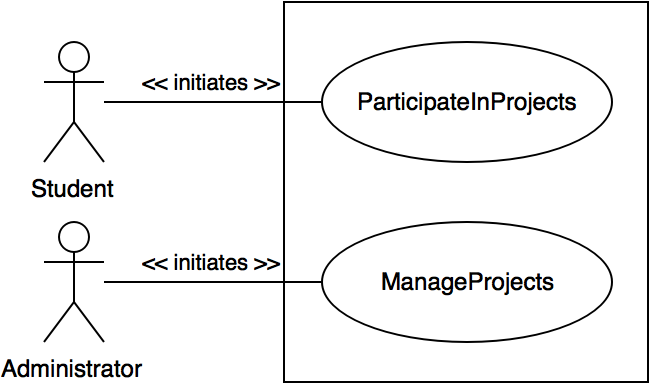
\includegraphics[scale=0.4]{imgs/high-level-use-case-diagram.png}
	\caption{High-level Use Case Diagram}
\end{figure}

\begin{table}[H]
	\caption{High-Level Use Case Descriptions}
	\vspace{1em}
	\begin{tabu} to \textwidth {l >{\bf}l X}
		UC-01 & ParticipateInProjects & The student accesses and can modify their own profile details (includes project participation details)\\
		UC-02 & ManageProjects & The Administrator manages current project as well as having the option to create a new instance of a 
		project (includes manipulating student participation and access to the PPID algorithm and its results). \\
	\end{tabu}
\end{table}

\begin{figure}[H]
	\centering{}
	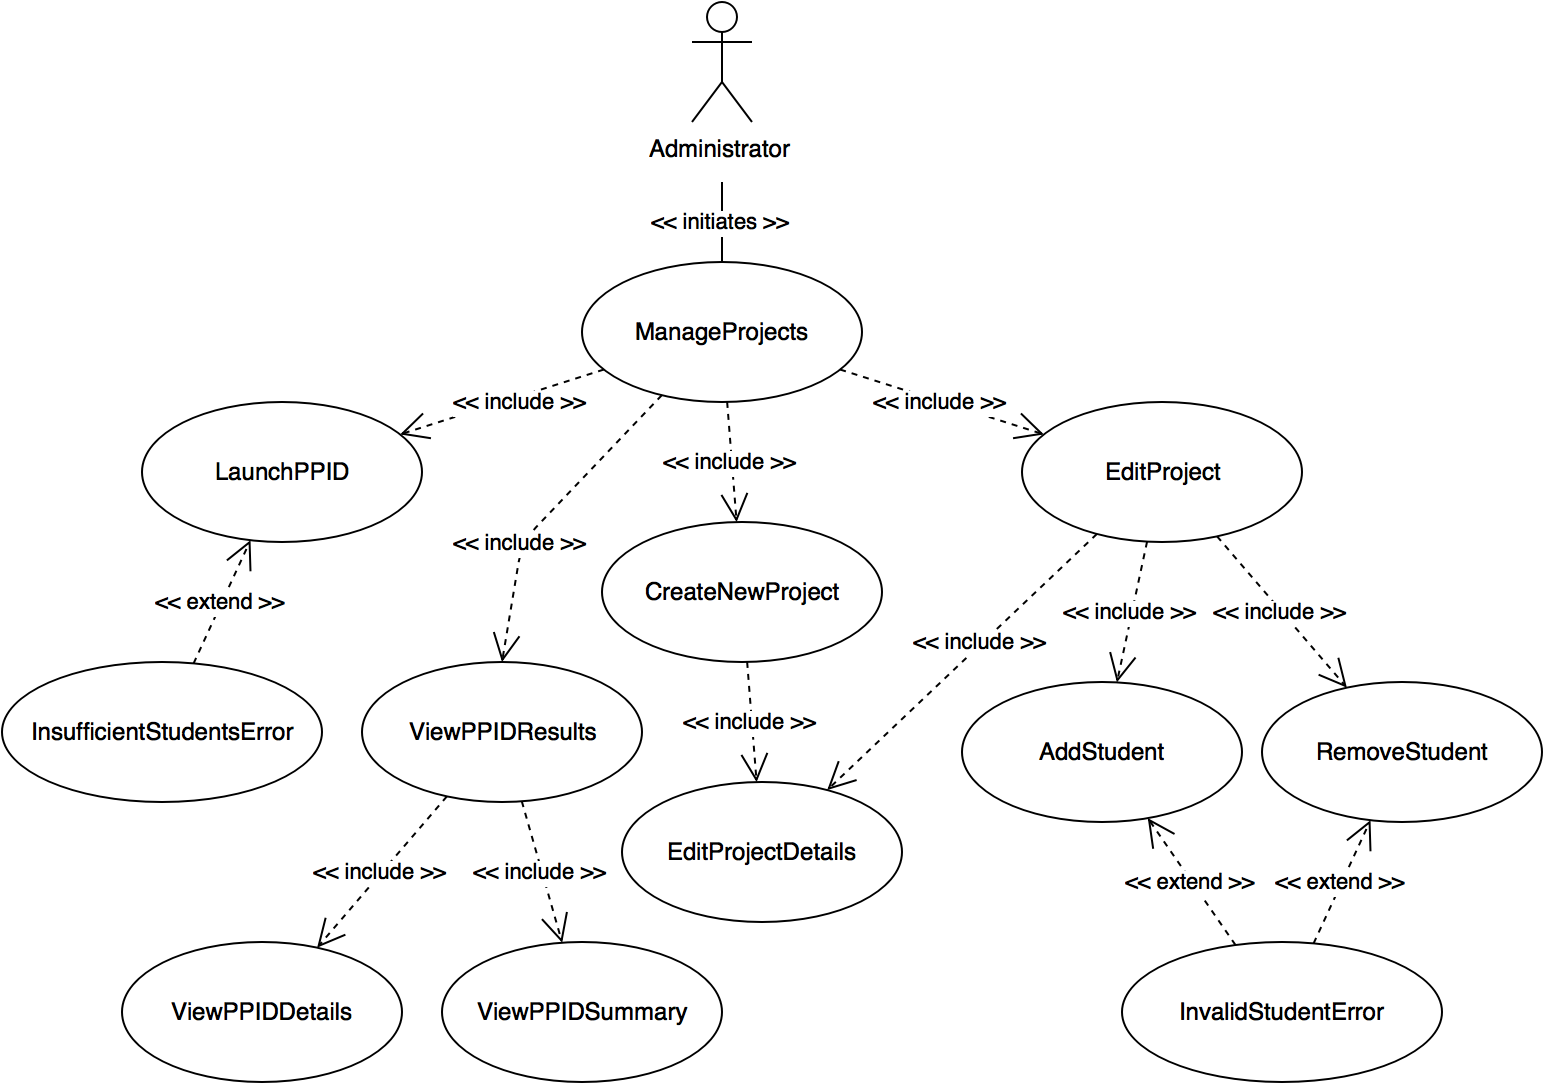
\includegraphics[scale=0.26]{imgs/detailed-administrator-use-case-diagram.png}
	\caption{Detailed Administrator Use Case Diagram}
\end{figure}

\begin{figure}[H]
	\centering{}
	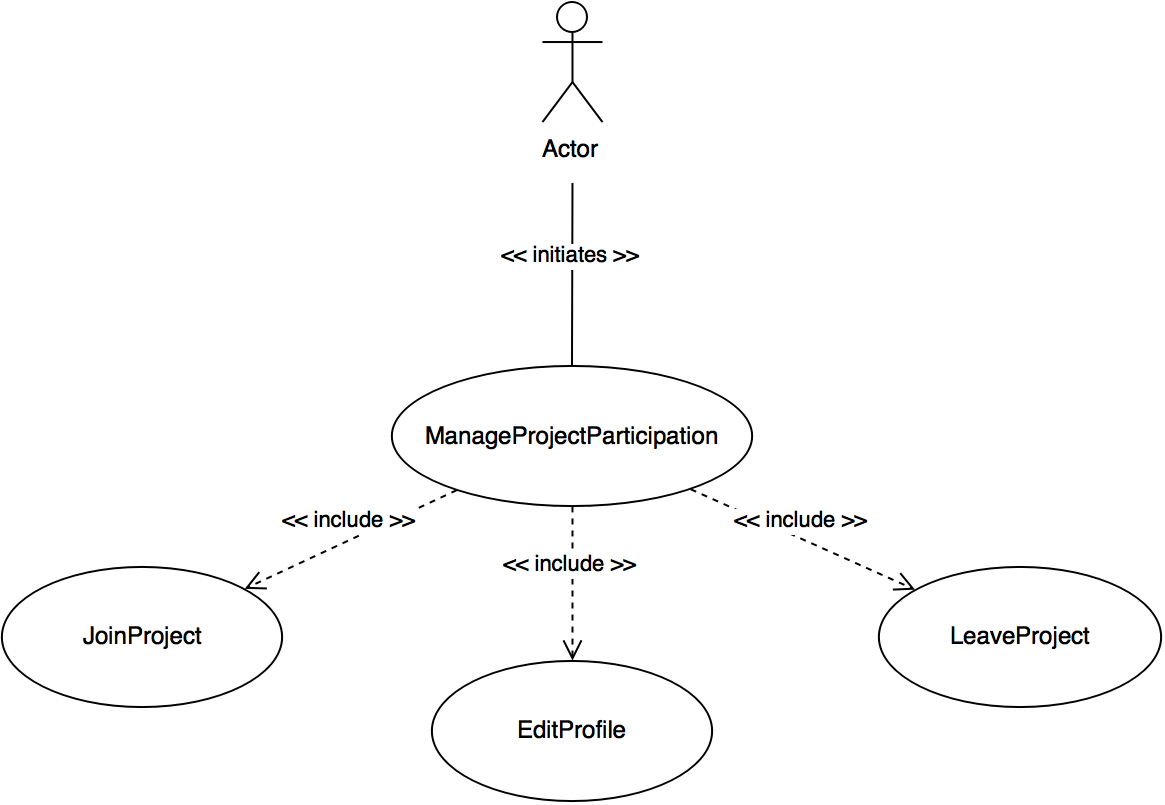
\includegraphics[scale=0.3]{imgs/detailed-student-use-case-diagram.png}
	\caption{Detailed Student Use Case Diagram}
\end{figure}

\begin{table}[H]
	\caption{Detailed Use Case Descriptions - Administrators}
	\vspace{1em}
	\begin{tabu} to \textwidth {l >{\bf}l X}
		UC-03 & ViewPPIDDetails & stuff\\
		UC-04 & CreateNewProject & The Administrator creates a new instance of a project.\\
		UC-05 & LaunchPPID & The Administrator applies the PPID Algorithm to a specified project.\\
		UC-06 & ViewPPIDSummary & stuff\\
		UC-07 & EditProject & The Administrator modifies the parameters of a specified project.\\
		UC-08 & AddStudent & The Administrator adds a Student to the current project.\\
		UC-09 & RemoveStudent & The Administrator removes a Student from the current project.\\
		UC-10 & SaveError & There was an error during saving (generalizes WriteError, ReadError, OpenError, CloseError). 
		The system reports the specific error to the user and aborts the operation.\\
		UC-11 & OpenError & The system reports that the selected file could not be opened.\\
		UC-12 & ReadError & The system reports that the selected file could not be read.\\
		UC-13 & WriteError & The system reports that the selected file could not be written to.\\
		UC-14 & CloseError & The system reports that the selected file could not be closed.\\
		UC-15 & InvalidInputError & The system reports that the given value is invalid.\\
		UC-16 & InvalidStudentError & The system reports that a student was not selected to carry out the selected operation on.\\
		UC-17 & InsufficientStudentsError & The system reports that there are not enough students registered in project to
		 run the PPID algorithm.\\
	\end{tabu}
\end{table}

\begin{table}[H]
	\caption{Detailed Use Case Descriptions - Students}
	\vspace{1em}
	\begin{tabu} to \textwidth {l >{\bf}l X}
		UC-18 & JoinProject & The student adds themselves to an existing project.\\
		UC-19 & EditProfile & The student modifies the parameters of their profile (includes EditPersonalValues and EditDesiredValues).\\
		UC-20 & LeaveProject & The student removes themselves from an existing project.\\
		UC-21 & EditPersonalValues & The student modifies the personal details in his profile (what they have to offer). \\
		UC-22 & EditDesiredValues & The student modifies the desired details in his profile (what they are looking for in potential team members). \\
	\end{tabu}
\end{table}

\begin{center}
	\begin{tabu} to \textwidth {>{\it}l X}
		\toprule
		Use Case Identifier & UC-01 \\
		Name & {\bf ParticipateInProjects} \\
		Participating Actors & Initiated by Student \\

		Flow of Events & 
	    \begin{enumerate}[topsep=-1em]
		    \item[1.] The Student begins the cuPID process
			\begin{enumerate}
				\item[2.] The Student is presented with a menu from the system. Options of: joining a project, leaving a project, or editing their profile for a project
			\end{enumerate}

		\end{enumerate} \\

		Entry Conditions &
		\begin{itemize}[topsep=-1em]
			\item  
        \end{itemize} \\

		Exit Conditions &
		\begin{itemize}[topsep=-1em]
			\item 
        \end{itemize} \\

		Quality Requirements &
		\begin{itemize}[topsep=-1em]
			\item 
        \end{itemize} \\

		Traceability & F-01, F-02, F-03, F-04\\

		\toprule
	\end{tabu}
\end{center}

\begin{center}
    \begin{tabu} to \textwidth {>{\it}l X}
        \toprule
		Use Case Identifier & UC-02 \\
		Name & {\bf ManageProjects} \\
        Participating Actors & Initiated by Administrato \\
		Flow of Events & 
	    \begin{enumerate}[topsep=-1em]
		    \item lots of stuff lots of stuff lots of stuff lots of stuff lots of stuff lots of stuff lots of stuff lots of stuff lots of stuff lots of stuff
		    \item other stuff lots of stuff lots of stuff lots of stuff lots of stuff lots of stuff lots of stuff lots of stuff
		\end{enumerate} \\

		Entry Conditions &
		\begin{itemize}[topsep=-1em]
		    \item lots of stuff lots of stuff lots of stuff lots of stuff lots of stuff lots of stuff lots of stuff lots of stuff lots of stuff lots of stuff
		    \item other stuff lots of stuff lots of stuff lots of stuff lots of stuff lots of stuff lots of stuff lots of stuff
        \end{itemize} \\

		Exit Conditions &
		\begin{itemize}[topsep=-1em]
		    \item lots of stuff lots of stuff lots of stuff lots of stuff lots of stuff lots of stuff lots of stuff lots of stuff lots of stuff lots of stuff
		    \item other stuff lots of stuff lots of stuff lots of stuff lots of stuff lots of stuff lots of stuff lots of stuff
        \end{itemize} \\

		Quality Requirements &
		\begin{itemize}[topsep=-1em]
		    \item lots of stuff lots of stuff lots of stuff lots of stuff lots of stuff lots of stuff lots of stuff lots of stuff lots of stuff lots of stuff
		    \item other stuff lots of stuff lots of stuff lots of stuff lots of stuff lots of stuff lots of stuff lots of stuff
        \end{itemize} \\

		Traceability & F-05, F-06, F-07, F-08, F-09\\
        \toprule
    \end{tabu}
\end{center}

\begin{center}
	\begin{tabu} to \textwidth {>{\it}l X}
		\toprule
		Use Case Identifier & UC-03 \\
		Name & {\bf ViewPPIDDetails} \\
		Participating Actors & Initiated by Administrato \\
		Flow of Events & 
	    \begin{enumerate}[topsep=-1em]
		    \item lots of stuff lots of stuff lots of stuff lots of stuff lots of stuff lots of stuff lots of stuff lots of stuff lots of stuff lots of stuff
		    \item other stuff lots of stuff lots of stuff lots of stuff lots of stuff lots of stuff lots of stuff lots of stuff
		\end{enumerate} \\

		Entry Conditions &
		\begin{itemize}[topsep=-1em]
		    \item lots of stuff lots of stuff lots of stuff lots of stuff lots of stuff lots of stuff lots of stuff lots of stuff lots of stuff lots of stuff
		    \item other stuff lots of stuff lots of stuff lots of stuff lots of stuff lots of stuff lots of stuff lots of stuff
        \end{itemize} \\

		Exit Conditions &
		\begin{itemize}[topsep=-1em]
		    \item lots of stuff lots of stuff lots of stuff lots of stuff lots of stuff lots of stuff lots of stuff lots of stuff lots of stuff lots of stuff
		    \item other stuff lots of stuff lots of stuff lots of stuff lots of stuff lots of stuff lots of stuff lots of stuff
        \end{itemize} \\

		Quality Requirements &
		\begin{itemize}[topsep=-1em]
		    \item lots of stuff lots of stuff lots of stuff lots of stuff lots of stuff lots of stuff lots of stuff lots of stuff lots of stuff lots of stuff
		    \item other stuff lots of stuff lots of stuff lots of stuff lots of stuff lots of stuff lots of stuff lots of stuff
        \end{itemize} \\

		Traceability & F-09 \\
		\toprule
	\end{tabu}
\end{center}

\begin{center}
	\begin{tabu} to \textwidth {>{\it}l X}
		\toprule
		Use Case Identifier & UC-04 \\
		Name & {\bf CreateNewProject} \\
		Participating Actors & Initiated by Administrato \\
		Flow of Events & 
	    \begin{enumerate}[topsep=-1em]
		    \item lots of stuff lots of stuff lots of stuff lots of stuff lots of stuff lots of stuff lots of stuff lots of stuff lots of stuff lots of stuff
		    \item other stuff lots of stuff lots of stuff lots of stuff lots of stuff lots of stuff lots of stuff lots of stuff
		\end{enumerate} \\

		Entry Conditions &
		\begin{itemize}[topsep=-1em]
		    \item lots of stuff lots of stuff lots of stuff lots of stuff lots of stuff lots of stuff lots of stuff lots of stuff lots of stuff lots of stuff
		    \item other stuff lots of stuff lots of stuff lots of stuff lots of stuff lots of stuff lots of stuff lots of stuff
        \end{itemize} \\

		Exit Conditions &
		\begin{itemize}[topsep=-1em]
		    \item lots of stuff lots of stuff lots of stuff lots of stuff lots of stuff lots of stuff lots of stuff lots of stuff lots of stuff lots of stuff
		    \item other stuff lots of stuff lots of stuff lots of stuff lots of stuff lots of stuff lots of stuff lots of stuff
        \end{itemize} \\

		Quality Requirements &
		\begin{itemize}[topsep=-1em]
		    \item lots of stuff lots of stuff lots of stuff lots of stuff lots of stuff lots of stuff lots of stuff lots of stuff lots of stuff lots of stuff
		    \item other stuff lots of stuff lots of stuff lots of stuff lots of stuff lots of stuff lots of stuff lots of stuff
        \end{itemize} \\

		Traceability & F-05 \\
		\toprule
	\end{tabu}
\end{center}

\begin{center}
	\begin{tabu} to \textwidth {>{\it}l X}
		\toprule
		Use Case Identifier & UC-05 \\
		Name & {\bf LaunchPPID} \\
		Participating Actors & Initiated by Administrato \\
		Flow of Events & 
	    \begin{enumerate}[topsep=-1em]
		    \item lots of stuff lots of stuff lots of stuff lots of stuff lots of stuff lots of stuff lots of stuff lots of stuff lots of stuff lots of stuff
		    \item other stuff lots of stuff lots of stuff lots of stuff lots of stuff lots of stuff lots of stuff lots of stuff
		\end{enumerate} \\

		Entry Conditions &
		\begin{itemize}[topsep=-1em]
		    \item lots of stuff lots of stuff lots of stuff lots of stuff lots of stuff lots of stuff lots of stuff lots of stuff lots of stuff lots of stuff
		    \item other stuff lots of stuff lots of stuff lots of stuff lots of stuff lots of stuff lots of stuff lots of stuff
        \end{itemize} \\

		Exit Conditions &
		\begin{itemize}[topsep=-1em]
		    \item lots of stuff lots of stuff lots of stuff lots of stuff lots of stuff lots of stuff lots of stuff lots of stuff lots of stuff lots of stuff
		    \item other stuff lots of stuff lots of stuff lots of stuff lots of stuff lots of stuff lots of stuff lots of stuff
        \end{itemize} \\

		Quality Requirements &
		\begin{itemize}[topsep=-1em]
		    \item lots of stuff lots of stuff lots of stuff lots of stuff lots of stuff lots of stuff lots of stuff lots of stuff lots of stuff lots of stuff
		    \item other stuff lots of stuff lots of stuff lots of stuff lots of stuff lots of stuff lots of stuff lots of stuff
        \end{itemize} \\

		Traceability & F-07 \\
		\toprule
	\end{tabu}
\end{center}

\begin{center}
	\begin{tabu} to \textwidth {>{\it}l X}
		\toprule
		Use Case Identifier & UC-06 \\
		Name & {\bf ViewPPIDSummary} \\
		Participating Actors & Initiated by Administrato \\
		Flow of Events & 
	    \begin{enumerate}[topsep=-1em]
		    \item lots of stuff lots of stuff lots of stuff lots of stuff lots of stuff lots of stuff lots of stuff lots of stuff lots of stuff lots of stuff
		    \item other stuff lots of stuff lots of stuff lots of stuff lots of stuff lots of stuff lots of stuff lots of stuff
		\end{enumerate} \\

		Entry Conditions &
		\begin{itemize}[topsep=-1em]
		    \item lots of stuff lots of stuff lots of stuff lots of stuff lots of stuff lots of stuff lots of stuff lots of stuff lots of stuff lots of stuff
		    \item other stuff lots of stuff lots of stuff lots of stuff lots of stuff lots of stuff lots of stuff lots of stuff
        \end{itemize} \\

		Exit Conditions &
		\begin{itemize}[topsep=-1em]
		    \item lots of stuff lots of stuff lots of stuff lots of stuff lots of stuff lots of stuff lots of stuff lots of stuff lots of stuff lots of stuff
		    \item other stuff lots of stuff lots of stuff lots of stuff lots of stuff lots of stuff lots of stuff lots of stuff
        \end{itemize} \\

		Quality Requirements &
		\begin{itemize}[topsep=-1em]
		    \item lots of stuff lots of stuff lots of stuff lots of stuff lots of stuff lots of stuff lots of stuff lots of stuff lots of stuff lots of stuff
		    \item other stuff lots of stuff lots of stuff lots of stuff lots of stuff lots of stuff lots of stuff lots of stuff
        \end{itemize} \\

		Traceability & F-08 \\
		\toprule
	\end{tabu}
\end{center}

\begin{center}
	\begin{tabu} to \textwidth {>{\it}l X}
		\toprule
		Use Case Identifier & UC-07 \\
		Name & {\bf EditProject} \\
		Participating Actors & Initiated by Administrato \\
		Flow of Events & 
	    \begin{enumerate}[topsep=-1em]
		    \item lots of stuff lots of stuff lots of stuff lots of stuff lots of stuff lots of stuff lots of stuff lots of stuff lots of stuff lots of stuff
		    \item other stuff lots of stuff lots of stuff lots of stuff lots of stuff lots of stuff lots of stuff lots of stuff
		\end{enumerate} \\

		Entry Conditions &
		\begin{itemize}[topsep=-1em]
		    \item lots of stuff lots of stuff lots of stuff lots of stuff lots of stuff lots of stuff lots of stuff lots of stuff lots of stuff lots of stuff
		    \item other stuff lots of stuff lots of stuff lots of stuff lots of stuff lots of stuff lots of stuff lots of stuff
        \end{itemize} \\

		Exit Conditions &
		\begin{itemize}[topsep=-1em]
		    \item lots of stuff lots of stuff lots of stuff lots of stuff lots of stuff lots of stuff lots of stuff lots of stuff lots of stuff lots of stuff
		    \item other stuff lots of stuff lots of stuff lots of stuff lots of stuff lots of stuff lots of stuff lots of stuff
        \end{itemize} \\

		Quality Requirements &
		\begin{itemize}[topsep=-1em]
		    \item lots of stuff lots of stuff lots of stuff lots of stuff lots of stuff lots of stuff lots of stuff lots of stuff lots of stuff lots of stuff
		    \item other stuff lots of stuff lots of stuff lots of stuff lots of stuff lots of stuff lots of stuff lots of stuff
        \end{itemize} \\

		Traceability & F-06 \\
		\toprule
	\end{tabu}
\end{center}

\begin{center}
	\begin{tabu} to \textwidth {>{\it}l X}
		\toprule
		Use Case Identifier & UC-08 \\
		Name & {\bf AddStudent} \\
		Participating Actors & Initiated by Administrato \\
		Flow of Events & 
	    \begin{enumerate}[topsep=-1em]
		    \item lots of stuff lots of stuff lots of stuff lots of stuff lots of stuff lots of stuff lots of stuff lots of stuff lots of stuff lots of stuff
		    \item other stuff lots of stuff lots of stuff lots of stuff lots of stuff lots of stuff lots of stuff lots of stuff
		\end{enumerate} \\

		Entry Conditions &
		\begin{itemize}[topsep=-1em]
		    \item lots of stuff lots of stuff lots of stuff lots of stuff lots of stuff lots of stuff lots of stuff lots of stuff lots of stuff lots of stuff
		    \item other stuff lots of stuff lots of stuff lots of stuff lots of stuff lots of stuff lots of stuff lots of stuff
        \end{itemize} \\

		Exit Conditions &
		\begin{itemize}[topsep=-1em]
		    \item lots of stuff lots of stuff lots of stuff lots of stuff lots of stuff lots of stuff lots of stuff lots of stuff lots of stuff lots of stuff
		    \item other stuff lots of stuff lots of stuff lots of stuff lots of stuff lots of stuff lots of stuff lots of stuff
        \end{itemize} \\

		Quality Requirements &
		\begin{itemize}[topsep=-1em]
		    \item lots of stuff lots of stuff lots of stuff lots of stuff lots of stuff lots of stuff lots of stuff lots of stuff lots of stuff lots of stuff
		    \item other stuff lots of stuff lots of stuff lots of stuff lots of stuff lots of stuff lots of stuff lots of stuff
        \end{itemize} \\

		Traceability & F-06-02 \\
		\toprule
	\end{tabu}
\end{center}

\begin{center}
	\begin{tabu} to \textwidth {>{\it}l X}
		\toprule
		Use Case Identifier & UC-09 \\
		Name & {\bf RemoveStudent} \\
		Participating Actors & Initiated by Administrator \\
		Flow of Events & 
	    \begin{enumerate}[topsep=-1em]
		    \item lots of stuff lots of stuff lots of stuff lots of stuff lots of stuff lots of stuff lots of stuff lots of stuff lots of stuff lots of stuff
		    \item other stuff lots of stuff lots of stuff lots of stuff lots of stuff lots of stuff lots of stuff lots of stuff
		\end{enumerate} \\

		Entry Conditions &
		\begin{itemize}[topsep=-1em]
		    \item lots of stuff lots of stuff lots of stuff lots of stuff lots of stuff lots of stuff lots of stuff lots of stuff lots of stuff lots of stuff
		    \item other stuff lots of stuff lots of stuff lots of stuff lots of stuff lots of stuff lots of stuff lots of stuff
        \end{itemize} \\

		Exit Conditions &
		\begin{itemize}[topsep=-1em]
		    \item lots of stuff lots of stuff lots of stuff lots of stuff lots of stuff lots of stuff lots of stuff lots of stuff lots of stuff lots of stuff
		    \item other stuff lots of stuff lots of stuff lots of stuff lots of stuff lots of stuff lots of stuff lots of stuff
        \end{itemize} \\

		Quality Requirements &
		\begin{itemize}[topsep=-1em]
		    \item lots of stuff lots of stuff lots of stuff lots of stuff lots of stuff lots of stuff lots of stuff lots of stuff lots of stuff lots of stuff
		    \item other stuff lots of stuff lots of stuff lots of stuff lots of stuff lots of stuff lots of stuff lots of stuff
        \end{itemize} \\

		Traceability & F-06-03 \\
		\toprule
	\end{tabu}
\end{center}

\begin{center}
	\begin{tabu} to \textwidth {>{\it}l X}
		\toprule
		Use Case Identifier & UC-10 \\
		Name & {\bf SaveError} \\
		Participating Actors & Administrator \\
		Flow of Events & 
	    \begin{enumerate}[topsep=-1em]
		    \item The system notifies the Administrator that an error has occured with regards to the processing of
		    the current file.
		\end{enumerate} \\

		Entry Conditions &
		\begin{itemize}[topsep=-1em]
		    \item A file processing operation failed.
        \end{itemize} \\

		Exit Conditions &
		\begin{itemize}[topsep=-1em]
		    \item The operation is aborted.
        \end{itemize} \\

		Quality Requirements &
		\begin{itemize}[topsep=-1em]
		    \item 
        \end{itemize} \\

		Traceability & NF-02 \\
		\toprule
	\end{tabu}
\end{center}

\begin{center}
	\begin{tabu} to \textwidth {>{\it}l X}
		\toprule
		Use Case Identifier & UC-11 \\
		Name & {\bf OpenError} \\
		Participating Actors & Administrator \\
		Flow of Events & 
	    \begin{enumerate}[topsep=-1em]
		    \item lots of stuff lots of stuff lots of stuff lots of stuff lots of stuff lots of stuff lots of stuff lots of stuff lots of stuff lots of stuff
		    \item other stuff lots of stuff lots of stuff lots of stuff lots of stuff lots of stuff lots of stuff lots of stuff
		\end{enumerate} \\

		Entry Conditions &
		\begin{itemize}[topsep=-1em]
		    \item lots of stuff lots of stuff lots of stuff lots of stuff lots of stuff lots of stuff lots of stuff lots of stuff lots of stuff lots of stuff
		    \item other stuff lots of stuff lots of stuff lots of stuff lots of stuff lots of stuff lots of stuff lots of stuff
        \end{itemize} \\

		Exit Conditions &
		\begin{itemize}[topsep=-1em]
		    \item lots of stuff lots of stuff lots of stuff lots of stuff lots of stuff lots of stuff lots of stuff lots of stuff lots of stuff lots of stuff
		    \item other stuff lots of stuff lots of stuff lots of stuff lots of stuff lots of stuff lots of stuff lots of stuff
        \end{itemize} \\

		Quality Requirements &
		\begin{itemize}[topsep=-1em]
		    \item lots of stuff lots of stuff lots of stuff lots of stuff lots of stuff lots of stuff lots of stuff lots of stuff lots of stuff lots of stuff
		    \item other stuff lots of stuff lots of stuff lots of stuff lots of stuff lots of stuff lots of stuff lots of stuff
        \end{itemize} \\

		Traceability & NF-02 \\
		\toprule
	\end{tabu}
\end{center}

\begin{center}
	\begin{tabu} to \textwidth {>{\it}l X}
		\toprule
		Use Case Identifier & UC-12 \\
		Name & {\bf ReadError} \\
		Participating Actors & Administrator \\
		Flow of Events & 
	    \begin{enumerate}[topsep=-1em]
		    \item lots of stuff lots of stuff lots of stuff lots of stuff lots of stuff lots of stuff lots of stuff lots of stuff lots of stuff lots of stuff
		    \item other stuff lots of stuff lots of stuff lots of stuff lots of stuff lots of stuff lots of stuff lots of stuff
		\end{enumerate} \\

		Entry Conditions &
		\begin{itemize}[topsep=-1em]
		    \item lots of stuff lots of stuff lots of stuff lots of stuff lots of stuff lots of stuff lots of stuff lots of stuff lots of stuff lots of stuff
		    \item other stuff lots of stuff lots of stuff lots of stuff lots of stuff lots of stuff lots of stuff lots of stuff
        \end{itemize} \\

		Exit Conditions &
		\begin{itemize}[topsep=-1em]
		    \item lots of stuff lots of stuff lots of stuff lots of stuff lots of stuff lots of stuff lots of stuff lots of stuff lots of stuff lots of stuff
		    \item other stuff lots of stuff lots of stuff lots of stuff lots of stuff lots of stuff lots of stuff lots of stuff
        \end{itemize} \\

		Quality Requirements &
		\begin{itemize}[topsep=-1em]
		    \item lots of stuff lots of stuff lots of stuff lots of stuff lots of stuff lots of stuff lots of stuff lots of stuff lots of stuff lots of stuff
		    \item other stuff lots of stuff lots of stuff lots of stuff lots of stuff lots of stuff lots of stuff lots of stuff
        \end{itemize} \\

		Traceability & NF-02 \\
		\toprule
	\end{tabu}
\end{center}

\begin{center}
	\begin{tabu} to \textwidth {>{\it}l X}
		\toprule
		Use Case Identifier & UC-13 \\
		Name & {\bf WriteError} \\
		Participating Actors & Administrator \\
		Flow of Events & 
	    \begin{enumerate}[topsep=-1em]
		    \item lots of stuff lots of stuff lots of stuff lots of stuff lots of stuff lots of stuff lots of stuff lots of stuff lots of stuff lots of stuff
		    \item other stuff lots of stuff lots of stuff lots of stuff lots of stuff lots of stuff lots of stuff lots of stuff
		\end{enumerate} \\

		Entry Conditions &
		\begin{itemize}[topsep=-1em]
		    \item lots of stuff lots of stuff lots of stuff lots of stuff lots of stuff lots of stuff lots of stuff lots of stuff lots of stuff lots of stuff
		    \item other stuff lots of stuff lots of stuff lots of stuff lots of stuff lots of stuff lots of stuff lots of stuff
        \end{itemize} \\

		Exit Conditions &
		\begin{itemize}[topsep=-1em]
		    \item lots of stuff lots of stuff lots of stuff lots of stuff lots of stuff lots of stuff lots of stuff lots of stuff lots of stuff lots of stuff
		    \item other stuff lots of stuff lots of stuff lots of stuff lots of stuff lots of stuff lots of stuff lots of stuff
        \end{itemize} \\

		Quality Requirements &
		\begin{itemize}[topsep=-1em]
		    \item lots of stuff lots of stuff lots of stuff lots of stuff lots of stuff lots of stuff lots of stuff lots of stuff lots of stuff lots of stuff
		    \item other stuff lots of stuff lots of stuff lots of stuff lots of stuff lots of stuff lots of stuff lots of stuff
        \end{itemize} \\

		Traceability & NF-02 \\
		\toprule
	\end{tabu}
\end{center}

\begin{center}
	\begin{tabu} to \textwidth {>{\it}l X}
		\toprule
		Use Case Identifier & UC-14 \\
		Name & {\bf CloseError} \\
		Participating Actors & Administrator \\
		Flow of Events & 
	    \begin{enumerate}[topsep=-1em]
		    \item lots of stuff lots of stuff lots of stuff lots of stuff lots of stuff lots of stuff lots of stuff lots of stuff lots of stuff lots of stuff
		    \item other stuff lots of stuff lots of stuff lots of stuff lots of stuff lots of stuff lots of stuff lots of stuff
		\end{enumerate} \\

		Entry Conditions &
		\begin{itemize}[topsep=-1em]
		    \item lots of stuff lots of stuff lots of stuff lots of stuff lots of stuff lots of stuff lots of stuff lots of stuff lots of stuff lots of stuff
		    \item other stuff lots of stuff lots of stuff lots of stuff lots of stuff lots of stuff lots of stuff lots of stuff
        \end{itemize} \\

		Exit Conditions &
		\begin{itemize}[topsep=-1em]
		    \item lots of stuff lots of stuff lots of stuff lots of stuff lots of stuff lots of stuff lots of stuff lots of stuff lots of stuff lots of stuff
		    \item other stuff lots of stuff lots of stuff lots of stuff lots of stuff lots of stuff lots of stuff lots of stuff
        \end{itemize} \\

		Quality Requirements &
		\begin{itemize}[topsep=-1em]
		    \item lots of stuff lots of stuff lots of stuff lots of stuff lots of stuff lots of stuff lots of stuff lots of stuff lots of stuff lots of stuff
		    \item other stuff lots of stuff lots of stuff lots of stuff lots of stuff lots of stuff lots of stuff lots of stuff
        \end{itemize} \\

		Traceability & NF-02 \\
		\toprule
	\end{tabu}
\end{center}

\begin{center}
	\begin{tabu} to \textwidth {>{\it}l X}
		\toprule
		Use Case Identifier & UC-15 \\
		Name & {\bf InvalidInputError} \\
		Participating Actors & Administrator \\
		Flow of Events & 
	    \begin{enumerate}[topsep=-1em]
		    \item lots of stuff lots of stuff lots of stuff lots of stuff lots of stuff lots of stuff lots of stuff lots of stuff lots of stuff lots of stuff
		    \item other stuff lots of stuff lots of stuff lots of stuff lots of stuff lots of stuff lots of stuff lots of stuff
		\end{enumerate} \\

		Entry Conditions &
		\begin{itemize}[topsep=-1em]
		    \item lots of stuff lots of stuff lots of stuff lots of stuff lots of stuff lots of stuff lots of stuff lots of stuff lots of stuff lots of stuff
		    \item other stuff lots of stuff lots of stuff lots of stuff lots of stuff lots of stuff lots of stuff lots of stuff
        \end{itemize} \\

		Exit Conditions &
		\begin{itemize}[topsep=-1em]
		    \item lots of stuff lots of stuff lots of stuff lots of stuff lots of stuff lots of stuff lots of stuff lots of stuff lots of stuff lots of stuff
		    \item other stuff lots of stuff lots of stuff lots of stuff lots of stuff lots of stuff lots of stuff lots of stuff
        \end{itemize} \\

		Quality Requirements &
		\begin{itemize}[topsep=-1em]
		    \item lots of stuff lots of stuff lots of stuff lots of stuff lots of stuff lots of stuff lots of stuff lots of stuff lots of stuff lots of stuff
		    \item other stuff lots of stuff lots of stuff lots of stuff lots of stuff lots of stuff lots of stuff lots of stuff
        \end{itemize} \\

		Traceability & NF-02 \\
		\toprule
	\end{tabu}
\end{center}

\begin{center}
	\begin{tabu} to \textwidth {>{\it}l X}
		\toprule
		Use Case Identifier & UC-16 \\
		Name & {\bf InvalidStudentError} \\
		Participating Actors & Administrator \\
		Flow of Events & 
	    \begin{enumerate}[topsep=-1em]
		    \item lots of stuff lots of stuff lots of stuff lots of stuff lots of stuff lots of stuff lots of stuff lots of stuff lots of stuff lots of stuff
		    \item other stuff lots of stuff lots of stuff lots of stuff lots of stuff lots of stuff lots of stuff lots of stuff
		\end{enumerate} \\

		Entry Conditions &
		\begin{itemize}[topsep=-1em]
		    \item lots of stuff lots of stuff lots of stuff lots of stuff lots of stuff lots of stuff lots of stuff lots of stuff lots of stuff lots of stuff
		    \item other stuff lots of stuff lots of stuff lots of stuff lots of stuff lots of stuff lots of stuff lots of stuff
        \end{itemize} \\

		Exit Conditions &
		\begin{itemize}[topsep=-1em]
		    \item lots of stuff lots of stuff lots of stuff lots of stuff lots of stuff lots of stuff lots of stuff lots of stuff lots of stuff lots of stuff
		    \item other stuff lots of stuff lots of stuff lots of stuff lots of stuff lots of stuff lots of stuff lots of stuff
        \end{itemize} \\

		Quality Requirements &
		\begin{itemize}[topsep=-1em]
		    \item lots of stuff lots of stuff lots of stuff lots of stuff lots of stuff lots of stuff lots of stuff lots of stuff lots of stuff lots of stuff
		    \item other stuff lots of stuff lots of stuff lots of stuff lots of stuff lots of stuff lots of stuff lots of stuff
        \end{itemize} \\

		Traceability & NF-02 \\
		\toprule
	\end{tabu}
\end{center}

\begin{center}
	\begin{tabu} to \textwidth {>{\it}l X}
		\toprule
		Use Case Identifier & UC-17 \\
		Name & {\bf InsufficientStudentsError} \\
		Participating Actors & Administrator \\
		Flow of Events & 
	    \begin{enumerate}[topsep=-1em]
		    \item lots of stuff lots of stuff lots of stuff lots of stuff lots of stuff lots of stuff lots of stuff lots of stuff lots of stuff lots of stuff
		    \item other stuff lots of stuff lots of stuff lots of stuff lots of stuff lots of stuff lots of stuff lots of stuff
		\end{enumerate} \\

		Entry Conditions &
		\begin{itemize}[topsep=-1em]
		    \item lots of stuff lots of stuff lots of stuff lots of stuff lots of stuff lots of stuff lots of stuff lots of stuff lots of stuff lots of stuff
		    \item other stuff lots of stuff lots of stuff lots of stuff lots of stuff lots of stuff lots of stuff lots of stuff
        \end{itemize} \\

		Exit Conditions &
		\begin{itemize}[topsep=-1em]
		    \item lots of stuff lots of stuff lots of stuff lots of stuff lots of stuff lots of stuff lots of stuff lots of stuff lots of stuff lots of stuff
		    \item other stuff lots of stuff lots of stuff lots of stuff lots of stuff lots of stuff lots of stuff lots of stuff
        \end{itemize} \\

		Quality Requirements &
		\begin{itemize}[topsep=-1em]
		    \item lots of stuff lots of stuff lots of stuff lots of stuff lots of stuff lots of stuff lots of stuff lots of stuff lots of stuff lots of stuff
		    \item other stuff lots of stuff lots of stuff lots of stuff lots of stuff lots of stuff lots of stuff lots of stuff
        \end{itemize} \\

		Traceability & NF-02 \\
		\toprule
	\end{tabu}
\end{center}

\begin{center}
	\begin{tabu} to \textwidth {>{\it}l X}
		\toprule
		Use Case Identifier & UC-18 \\
		Name & {\bf JoinProject} \\
		Participating Actors & Initiated by Student \\
		Flow of Events & 
	    \begin{enumerate}[topsep=-1em]
		    \item lots of stuff lots of stuff lots of stuff lots of stuff lots of stuff lots of stuff lots of stuff lots of stuff lots of stuff lots of stuff
		    \item other stuff lots of stuff lots of stuff lots of stuff lots of stuff lots of stuff lots of stuff lots of stuff
		\end{enumerate} \\

		Entry Conditions &
		\begin{itemize}[topsep=-1em]
		    \item lots of stuff lots of stuff lots of stuff lots of stuff lots of stuff lots of stuff lots of stuff lots of stuff lots of stuff lots of stuff
		    \item other stuff lots of stuff lots of stuff lots of stuff lots of stuff lots of stuff lots of stuff lots of stuff
        \end{itemize} \\

		Exit Conditions &
		\begin{itemize}[topsep=-1em]
		    \item lots of stuff lots of stuff lots of stuff lots of stuff lots of stuff lots of stuff lots of stuff lots of stuff lots of stuff lots of stuff
		    \item other stuff lots of stuff lots of stuff lots of stuff lots of stuff lots of stuff lots of stuff lots of stuff
        \end{itemize} \\

		Quality Requirements &
		\begin{itemize}[topsep=-1em]
		    \item lots of stuff lots of stuff lots of stuff lots of stuff lots of stuff lots of stuff lots of stuff lots of stuff lots of stuff lots of stuff
		    \item other stuff lots of stuff lots of stuff lots of stuff lots of stuff lots of stuff lots of stuff lots of stuff
        \end{itemize} \\

		Traceability & NF-02 \\
		\toprule
	\end{tabu}
\end{center}

\begin{center}
	\begin{tabu} to \textwidth {>{\it}l X}
		\toprule
		Use Case Identifier & UC-19 \\
		Name & {\bf EditProfile} \\
		Participating Actors & Initiated by Student \\
		Flow of Events & 
	    \begin{enumerate}[topsep=-1em]
		    \item lots of stuff lots of stuff lots of stuff lots of stuff lots of stuff lots of stuff lots of stuff lots of stuff lots of stuff lots of stuff
		    \item other stuff lots of stuff lots of stuff lots of stuff lots of stuff lots of stuff lots of stuff lots of stuff
		\end{enumerate} \\

		Entry Conditions &
		\begin{itemize}[topsep=-1em]
		    \item lots of stuff lots of stuff lots of stuff lots of stuff lots of stuff lots of stuff lots of stuff lots of stuff lots of stuff lots of stuff
		    \item other stuff lots of stuff lots of stuff lots of stuff lots of stuff lots of stuff lots of stuff lots of stuff
        \end{itemize} \\

		Exit Conditions &
		\begin{itemize}[topsep=-1em]
		    \item lots of stuff lots of stuff lots of stuff lots of stuff lots of stuff lots of stuff lots of stuff lots of stuff lots of stuff lots of stuff
		    \item other stuff lots of stuff lots of stuff lots of stuff lots of stuff lots of stuff lots of stuff lots of stuff
        \end{itemize} \\

		Quality Requirements &
		\begin{itemize}[topsep=-1em]
		    \item lots of stuff lots of stuff lots of stuff lots of stuff lots of stuff lots of stuff lots of stuff lots of stuff lots of stuff lots of stuff
		    \item other stuff lots of stuff lots of stuff lots of stuff lots of stuff lots of stuff lots of stuff lots of stuff
        \end{itemize} \\

		Traceability & NF-02 \\
		\toprule
	\end{tabu}
\end{center}

\begin{center}
	\begin{tabu} to \textwidth {>{\it}l X}
		\toprule
		Use Case Identifier & UC-20 \\
		Name & {\bf LeaveProject} \\
		Participating Actors & Initiated by Student \\
		Flow of Events & 
	    \begin{enumerate}[topsep=-1em]
		    \item lots of stuff lots of stuff lots of stuff lots of stuff lots of stuff lots of stuff lots of stuff lots of stuff lots of stuff lots of stuff
		    \item other stuff lots of stuff lots of stuff lots of stuff lots of stuff lots of stuff lots of stuff lots of stuff
		\end{enumerate} \\

		Entry Conditions &
		\begin{itemize}[topsep=-1em]
		    \item lots of stuff lots of stuff lots of stuff lots of stuff lots of stuff lots of stuff lots of stuff lots of stuff lots of stuff lots of stuff
		    \item other stuff lots of stuff lots of stuff lots of stuff lots of stuff lots of stuff lots of stuff lots of stuff
        \end{itemize} \\

		Exit Conditions &
		\begin{itemize}[topsep=-1em]
		    \item lots of stuff lots of stuff lots of stuff lots of stuff lots of stuff lots of stuff lots of stuff lots of stuff lots of stuff lots of stuff
		    \item other stuff lots of stuff lots of stuff lots of stuff lots of stuff lots of stuff lots of stuff lots of stuff
        \end{itemize} \\

		Quality Requirements &
		\begin{itemize}[topsep=-1em]
		    \item lots of stuff lots of stuff lots of stuff lots of stuff lots of stuff lots of stuff lots of stuff lots of stuff lots of stuff lots of stuff
		    \item other stuff lots of stuff lots of stuff lots of stuff lots of stuff lots of stuff lots of stuff lots of stuff
        \end{itemize} \\

		Traceability & NF-02 \\
		\toprule
	\end{tabu}
\end{center}

\subsubsection{Object Model}


\subsubsection{Dynamic Model}


\end{document}
